\documentclass[a4paper,12pt]{article}

\usepackage[utf8]{inputenc}
\usepackage[english]{babel}
\usepackage[T1]{fontenc} % for correct << and >>
\usepackage{amssymb, amsmath, multicol, amsthm, mathtools}
\usepackage{csquotes}
\usepackage{mathrsfs}
\usepackage{graphicx}
\usepackage{multirow}
\usepackage{caption}
\usepackage{subcaption}
\usepackage{indentfirst}
\usepackage{esvect}
\usepackage{float} 
\usepackage[version=4]{mhchem}
\mathtoolsset{showonlyrefs=true}
\usepackage{hyperref}
\usepackage[rgb,table,xcdraw]{xcolor}
\hypersetup{				
	unicode=true,        
	colorlinks=true,       	
	linkcolor=black,        
	citecolor=black,        
	filecolor=magenta,      
	urlcolor=black         
}
\usepackage{pythonhighlight}

\usepackage[left=2cm,right=2cm,
    top=2cm,bottom=2cm]{geometry}
\usepackage{fancyhdr}


\graphicspath{{images}}

\newcommand{\angstrom}{\text{\normalfont\AA}}
\newcommand{\iu}{\mathrm{i}\mkern1mu}
\newcommand*{\hatH}{\hat{\mathcal{H}}}


\newcommand{\highlightgreen}[1]{%
  \colorbox{green!50}{$\displaystyle#1$}}
  \newcommand{\highlightblue}[1]{%
  \colorbox{blue!50}{$\displaystyle#1$}}


\begin{document}

    \begin{center}
    \centering \LARGE SpinW factor 2 problem

    \vspace{1cm}
    \small Andrey Rybakov and Marco Marino
    \end{center}

    \section{The problem}

        SpinW \cite{SpinW} results does not reproduce the test case of 1D ferromagnetic chain, neither 3D ferromagnetic cubic crystal. 
        The magnon dispersion for such systems plotted with SpinW is twice as small as the result from textbooks 
        \cite{rezende2020fundamentals, blundell2003magnetism, gurevich1996magnetization, simon2013oxford, coey2010magnetism, jensen1991rare, white1983quantum} (conversion from textbook's notations are discussed in Appendix~I). 

        Since there are various notations for the spin hamiltonian, which is the starting point for the magnon dispersion calculation, 
        in this paper all results are presents with respect to the notation of SpinW paper \cite{toth2015linear}:

        \begin{equation}
            H = \sum_{mi,nj}\boldsymbol{S}^T_{mi}\boldsymbol{J}_{mi, nj}\boldsymbol{S}_{nj} + 
            \sum_{mi}\boldsymbol{S}^T_{mi}\boldsymbol{A}_{mi}\boldsymbol{S}_{mi} + 
            \mu_B\boldsymbol{H}^T\sum_{mi}g_i\boldsymbol{S}_{mi},
        \end{equation}
        where double counting is present in the sum and negative $J$ means ferromagnetic alignment. 
        First term describes exchange interaction, second -- single ion anisotropy, third -- external magnetic field.
        The indices $m$, $n$ are indexing the crystallographic unit cell (running from $1$ to $L$), while $i$ and $j$ label the magnetic atoms inside unit cell (running from $1$ to $N$).
        $\boldsymbol{S}_i$ is a $3 \times 1$ column vector of spin operators $\{S_{mi}^x, S_{mi}^y, S_{mi}^z\}$, 
        $\boldsymbol{J}_{mi, nj}$ is a matrix of exchange parameters, $\boldsymbol{A}_{mi}$ - matrix of single ion anisotropy,  
        $\boldsymbol{H}$ - column vector of external magnetic field. 

        For the ferromagnetic 3D crystal with one magnetic center in unit cell the solution of SpinW is:

        \begin{equation}
            E(\boldsymbol{k}) = \hbar\omega(\boldsymbol{k}) = SJn\left(\dfrac{1}{3}\left(\cos(k_xl) + \cos(k_yl) + \cos(k_zl)\right) - 1\right),
        \end{equation}
        where $l$ is the length of lattice parameters. While the textbook's results for the same system are:
        \begin{equation}
            E(\boldsymbol{k}) = \hbar\omega(\boldsymbol{k}) = 2SJn\left(\dfrac{1}{3}\left(\cos(k_xl) + \cos(k_yl) + \cos(k_zl)\right) - 1\right). \label{eq:textbook}
        \end{equation}

        In the Fig.~\ref{fig:dispersion-comparasion} The magnon dispersion is plotted for both solutions along the k-path specified in \cite{setyawan2010high}, $J = 1$, $S = 1$, $n = 6$.

        \begin{figure}[H]
            \centering
            \begin{subfigure}[b]{0.8\textwidth}
                \centering
                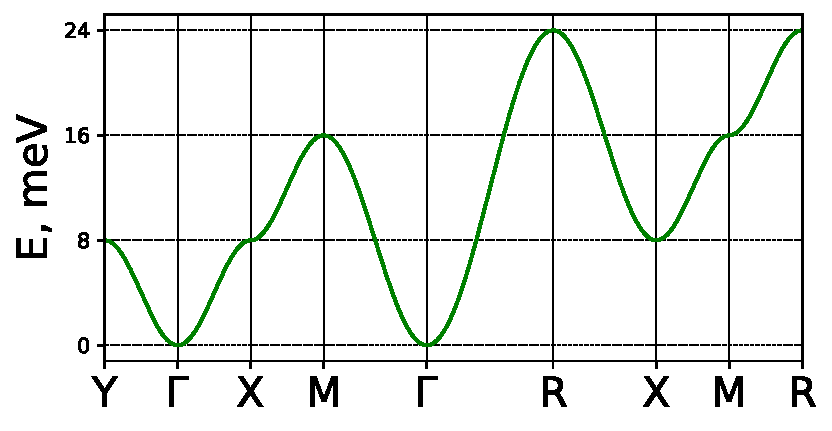
\includegraphics[height=6cm]{main_dispersion.pdf}
            \end{subfigure}
            \hfill
            \caption{Magnon dispersion comparison between SpinW and textbooks ($J = 1$, $S = 1$).}
            \label{fig:dispersion-comparasion}
        \end{figure}

        In the SpinW paper \cite{toth2015linear} the solution starts by the two consecutive rotations, 
        One results in the rotation of the exchange matrix $\boldsymbol{J}^{\prime}_{mi, nj} = \boldsymbol{J}_{mi, nj}\boldsymbol{R}_{n-m}$ 
        and another defines the vectors $\boldsymbol{u}$ and $\boldsymbol{v}$.
        These rotations do not affect the following discussion, therefore we drop the $^{\prime}$ sign in the $\boldsymbol{J}^{\prime}_{mi, nj}$ 
        and use the complex valued vectors $\boldsymbol{u}$ and $\boldsymbol{v}$, without recalling their definition. 
        The unique comment that is important here is that for ferromagnetic case (oriented along $z$ axis) the values of the vectors are:
        \begin{equation}
            \boldsymbol{u} = (1, i, 0)^T
        \end{equation}
        \begin{equation}
            \boldsymbol{v} = (0, 0, 1)^T
        \end{equation}

        The single-ion anisotropy and magnetic field can be merged into the exchange term as explained in the SpinW paper \cite{toth2015linear}.

    \section{The solution}

        Starting point for the following discussion is equation (20) from the SpinW paper \cite{toth2015linear} 
        (adjusted with respect to the comment at the end of the previous section):

        \begin{multline}
            H = \sum_{mi, nj}\left\{\sqrt{\dfrac{S_{i}}{2}}\left(\overline{\boldsymbol{u}}^T_i b_{mi} + \boldsymbol{u}^T_i b^{\dag}_{mi} \right) + 
            \boldsymbol{v}^T_i(S_i - b^{\dag}_{mi}b_{mi})\right\}  \cdot
            \boldsymbol{J}_{mi, nj}\\
            \cdot\left\{\sqrt{\dfrac{S_{j}}{2}}\left(\overline{\boldsymbol{u}}_j b_{nj} + \boldsymbol{u}_j b^{\dag}_{nj} \right) + 
            \boldsymbol{v}_j(S_j - b^{\dag}_{nj}b_{nj})\right\},
        \end{multline}
        where $b^{\dag}_{mi}$ and $b_{mi}$ are the creation and annihilation operators of the local quantum spin deviations. Overline denotes complex conjugate.

        After the expansion the Hamiltonian has the zero energy term $E_0$, the one-operator terms, 
        and the two-operator term $H^{(2)}$, which is the center of attention in linearised spin-wave theory. 
        We focus on this term, taking into account the property of the exchange matrix $\boldsymbol{J}_{mi, nj} = \boldsymbol{J}_{i,j}(d)$, $\boldsymbol{d} = \boldsymbol{r}_n - \boldsymbol{r}_m$:
        \begin{multline}
            H^{(2)} = \dfrac{\sqrt{S_i S_j}}{2}\left(\overline{\boldsymbol{u}}^T_i\boldsymbol{J}_{i,j}(\boldsymbol{d})\overline{\boldsymbol{u}}_jb_{mi}b_{nj} +
            \overline{\boldsymbol{u}}^T_i\boldsymbol{J}_{i,j}(\boldsymbol{d})\boldsymbol{u}_j b_{mi}b^{\dag}_{nj}\right. \\+ 
            \left.\boldsymbol{u}^T_i\boldsymbol{J}_{i,j}(\boldsymbol{d})\overline{\boldsymbol{u}}_jb^{\dag}_{mi}b_{nj} +
            \boldsymbol{u}^T_i\boldsymbol{J}_{i,j}(\boldsymbol{d})\boldsymbol{u}_jb^{\dag}_{mi}b^{\dag}_{nj}\right) \\-
            \boldsymbol{v}^T_i\boldsymbol{J}_{i,j}(\boldsymbol{d})\boldsymbol{v}_j\left(S_ib^{\dag}_{nj}b_{nj} + S_jb^{\dag}_{mi}b_{mi}\right)
        \end{multline}

        The next step of the solution is to apply Fourier transformation in order to move from the creation and annihilation operators 
        of the local quantum spin deviations ($b^{\dag}_{mi}$ and $b_{mi}$) 
        to the creation and annihilation operators of the collective quantum excitations ($b^{\dag}(k)$ and $b(k)$).
        \begin{equation}
            b_{mi} = \dfrac{1}{\sqrt{L}}\sum_{\boldsymbol{k} \in \text{B.Z.}} b_i(\boldsymbol{k})e^{i\boldsymbol{k}\boldsymbol{r}_m},
        \end{equation}
        \begin{equation}
            b^{\dag}_{mi} = \dfrac{1}{\sqrt{L}}\sum_{\boldsymbol{k} \in \text{B.Z.}} b^{\dag}_i(\boldsymbol{k})e^{-i\boldsymbol{k}\boldsymbol{r}_m},
        \end{equation}

        After the Fourier transformation the Hamiltonian has the form:
        \begin{multline}
            H^{(2)} = \sum_{ij}\sum_{\boldsymbol{k}}\left[\dfrac{\sqrt{S_i S_j}}{2}\overline{\boldsymbol{u}}^T_i\boldsymbol{J}_{i,j}(\boldsymbol{k})\overline{\boldsymbol{u}}_jb_{i}(\boldsymbol{k})b_{j}(-\boldsymbol{k}) +
            \dfrac{\sqrt{S_i S_j}}{2} \overline{\boldsymbol{u}}^T_i\boldsymbol{J}_{i,j}(\boldsymbol{k})\boldsymbol{u}_j b_{i}(\boldsymbol{k})b^{\dag}_{j}(\boldsymbol{k})\right. \\+ 
            \dfrac{\sqrt{S_i S_j}}{2}\boldsymbol{u}^T_i\boldsymbol{J}_{i,j}(-\boldsymbol{k})\overline{\boldsymbol{u}}_jb^{\dag}_{i}(\boldsymbol{k})b_{j}(\boldsymbol{k}) +
            \dfrac{\sqrt{S_i S_j}}{2}\boldsymbol{u}^T_i\boldsymbol{J}_{i,j}(-\boldsymbol{k})\boldsymbol{u}_jb^{\dag}_{i}(\boldsymbol{k})b^{\dag}_{j}(-\boldsymbol{k}) \\-
            \left.S_i\boldsymbol{v}^T_i\boldsymbol{J}_{i,j}(\boldsymbol{0})\boldsymbol{v}_jb^{\dag}_{j}(\boldsymbol{k})b_{j}(\boldsymbol{k}) + 
            S_j\boldsymbol{v}^T_i\boldsymbol{J}_{i,j}(\boldsymbol{0})\boldsymbol{v}_jb^{\dag}_{i}(\boldsymbol{k})b_{i}(\boldsymbol{k})\right]
        \end{multline}

        We follow the definitions from the equation (26) of the SpinW paper \cite{toth2015linear}:
        \begin{equation}
            \boldsymbol{J}_{i,j}(\boldsymbol{k}) = \sum_{\boldsymbol{d}}\boldsymbol{J}_{i,j}(\boldsymbol{d})e^{-i\boldsymbol{k}\boldsymbol{d}}
        \end{equation}
        \begin{equation}
            A(\boldsymbol{k})^{i,j} = \dfrac{\sqrt{S_i, S_j}}{2}\boldsymbol{u}^T_i\boldsymbol{J}_{i,j}(-\boldsymbol{k})\overline{\boldsymbol{u}}_j,
        \end{equation}
        \begin{equation}
            B(\boldsymbol{k})^{i,j} = \dfrac{\sqrt{S_i, S_j}}{2}\boldsymbol{u}^T_i\boldsymbol{J}_{i,j}(-\boldsymbol{k})\boldsymbol{u}_j,
        \end{equation}
        \begin{equation}
            C(\boldsymbol{k})^{i,j} = C^{i,j} = \delta_{i,j}\sum_{l}S_l \boldsymbol{v}^T_i\boldsymbol{J}_{i, l}(\boldsymbol{0})\boldsymbol{v}_l.
        \end{equation}

        With this notation the Hamiltonian becomes:
        \begin{multline}
            H^{(2)} = \sum_{ij}\sum_{\boldsymbol{k}}\left[\overline{B^{i,j}(\boldsymbol{k})}b_{i}(\boldsymbol{k})b_{j}(-\boldsymbol{k}) +
            \overline{A^{i,j}(\boldsymbol{k})}b_{i}(\boldsymbol{k})b^{\dag}_{j}(\boldsymbol{k})\right. \\+ 
            A^{i,j}(\boldsymbol{k})b^{\dag}_{i}(\boldsymbol{k})b_{j}(\boldsymbol{k}) +
            B^{i,j}(\boldsymbol{k})b^{\dag}_{i}(\boldsymbol{k})b^{\dag}_{j}(-\boldsymbol{k}) \\-
            \left.2 C^{i,j}b^{\dag}_{i}(\boldsymbol{k})b_{j}(\boldsymbol{k})\right] \label{eq:ham-before}
        \end{multline}

        It is important to note, that the Hamiltonian \eqref{eq:ham-before} is the last point before the solution of SpinW paper \cite{toth2015linear} 
        differs from the solution of Colpa (subsection~\ref{sec:colpa}) or White and Bayne (subsection~\ref{sec:white}).

        Next step is to rewrite the Hamiltonian in the quadratic form:
        \begin{equation}
            H = \sum_{\boldsymbol{k} ?} \boldsymbol{x}^{\dag}(\boldsymbol{k})h(\boldsymbol{k})\boldsymbol{x}(\boldsymbol{k}), \label{eq:quadratic-form}
        \end{equation}
        where
        \begin{equation}
            \boldsymbol{x}(\boldsymbol{k}) = \left[b_1(\boldsymbol{k}), \dots, b_N(\boldsymbol{k}), 
            b^{\dag}_1(-\boldsymbol{k}), \dots, b^{\dag}_N(-\boldsymbol{k})\right]^T
        \end{equation}
        and (in the SpinW paper \cite{toth2015linear})
        \begin{equation}
            h(\boldsymbol{k}) = 
            \begin{pmatrix}
                \boldsymbol{A}(\boldsymbol{k}) - \boldsymbol{C} & \boldsymbol{B}(\boldsymbol{k}) \\
                \boldsymbol{B}^{\dag}(\boldsymbol{k}) &\overline{\boldsymbol{A}(-\boldsymbol{k})} - \boldsymbol{C} \\
            \end{pmatrix} \label{eq:h-spinw}
        \end{equation}
        where $^{\dag}$ means hermitian conjugate.
        
        There is a question mark near the $\boldsymbol{k}$ under the sum, since that is the place where SpinW solution and what we are going to do next differ.
        In the article of Colpa \cite{colpa1978diagonalization}, in the textbook by Rezende \cite{rezende2020fundamentals} (page~$83$) 
        and indirectly in the article of White \cite{white1965diagonalization}, textbook \cite{jensen1991rare} the restriction $\boldsymbol{k} > 0$ is implied, 
        which means that for each $\boldsymbol{k}$ in the sum $-\boldsymbol{k}$ is not in the sum (it is not in the set of indexes over which the sum is carried out). 
        Alternatively, in the textbook by White \cite{white1983quantum} 
        the factor $1/2$ added in front of the quadratic Hamiltonian \eqref{eq:quadratic-form} with no restriction to $\boldsymbol{k}$, 
        which leads to the same result as with the restriction on $\boldsymbol{k}$ mentioned above.

        However, SpinW paper \cite{toth2015linear} proceeds to cast the Hamiltonian \eqref{eq:ham-before} into quadratic form \eqref{eq:quadratic-form} without any restriction on $\boldsymbol{k}$,
        moreover, it is specifically noted under the sum in equation 23 that $\boldsymbol{k} \in \text{B.Z.}$. 

        In the SpinW paper the diagonalization of the quadratic form \eqref{eq:quadratic-form} follows the method by Colpa \cite{colpa1978diagonalization}. 
        In the code itself the diagonalization method by White \cite{white1983quantum} is mentioned.
        Let us compare the starting points of Colpa and White with SpinW before diagonalization. 

        In the Hamiltonian \eqref{eq:ham-before} only the part for the $\boldsymbol{k}$ is written explicitly for each $\boldsymbol{k}$ under the sum. 
        Therefore one needs to add terms for $-\boldsymbol{k}$ in order to construct the form \eqref{eq:ham-colpa}. 
        There are two ways to do that:

        \begin{itemize}
            \item To restrict ourselves to the $\boldsymbol{k} > 0$ and rewrite the Hamiltonian. 
            This approach can be interpreted as the separation of the space into $\boldsymbol{k} > 0$ and $\boldsymbol{k} < 0$ parts and the solution. 
            We focus on this approach in the subsection~\ref{sec:colpa}, where we follow the solution of Colpa \cite{colpa1978diagonalization}.

            \item To keep the whole set of $\boldsymbol{k}$ and add $\sum_{-\boldsymbol{k}}$ to the Hamiltonian.
            This approach can be interpreted as the artificial addition of the Hamiltonian with the magnons propagating back in time for every $\boldsymbol{k}$.
            We discuss this approach in the subsection~\ref{sec:white}, where we follow the solution of White and Bayne \cite{white1983quantum}.
        \end{itemize}

        The source of the problem with the equation \eqref{eq:h-spinw} is discussed in the subsection~\ref{sec:spinw}.
        
        \subsection{Colpa \cite{colpa1978diagonalization}}\label{sec:colpa}
        
            Colpa discusses the diagonalization of the Bogoliubov Hamiltonian of the form:

            \begin{equation}
                H = \sum_{r^{\prime}, r = 1}^m \left(\alpha_{r^{\prime}}^{\dag}\Delta_{1r^{\prime}r}\alpha_r +
                \alpha_{r^{\prime}}^{\dag}\Delta_{2r^{\prime}r}\alpha_{m+r}^{\dag} +
                \alpha_{m + r^{\prime}}\Delta_{3r^{\prime}r}\alpha_r +
                \alpha_{m + r^{\prime}}\Delta_{4r^{\prime}r}\alpha_{m + r}^{\dag}\right), \label{eq:ham-colpa}
            \end{equation}
            with the following comment on the possible nature of the indices $r$ and $m+r$:
            \begin{quote}
                The reason why we consider first eq $(2.1)$ is that it often occurs in practice 
                [in solid-state physics e.g. all operators with indes $r$ correspond to the same wave vector $\boldsymbol{k}$, 
                those with $m+r$ to $-\boldsymbol{k}$; $m$ denotes the number of degrees of freedom in the unit cell (or less)] 
            \end{quote}

            We have just the case of the solid-state physics. Note, that in the Hamiltonian \eqref{eq:ham-colpa} the sum is carried out over $m$ and not $2m$, 
            which means that in the sum the terms with $\boldsymbol{k}$ and $-\boldsymbol{k}$ are written explicitly. 

            First of all, we write the Hamiltonian in a more compact form:
            \begin{multline}
                H^{(2)} = \sum_{ij}\sum_{\boldsymbol{k}}\left[2(A^{i,j}(\boldsymbol{k}) - C^{i,j})b^{\dag}_{i}(\boldsymbol{k})b_{j}(\boldsymbol{k}) + 
                \overline{B^{i,j}(\boldsymbol{k})}b_{i}(\boldsymbol{k})b_{j}(-\boldsymbol{k}) +
                B^{i,j}(\boldsymbol{k})b^{\dag}_{i}(\boldsymbol{k})b^{\dag}_{j}(-\boldsymbol{k})\right]\\
                +\sum_i \sum_{\boldsymbol{k}} A^{i,i}(\boldsymbol{k}) 
                = \sum_{ij}\sum_{\boldsymbol{k}} H^{i,j}(\boldsymbol{k}) 
                + const, \label{eq:ham-simple}
            \end{multline}
            where we used the fact that $\boldsymbol{A}(\boldsymbol{k})$ is Hermitian (see Appendix II) and the commutator $[b_{i}(\boldsymbol{k})b^{\dag}_{j}(\boldsymbol{k})] = \delta_{i,j}$. 
            In the following we omit the terms of the constant energy shift. Next tep is to imply constrain of $\boldsymbol{k}>0$:

            \begin{multline}
                H^{(2)} = \sum_{ij}\sum_{\boldsymbol{k} > 0} \left(H^{i,j}(\boldsymbol{k}) + H^{i,j}(-\boldsymbol{k})\right) \\
                = \sum_{ij}\sum_{\boldsymbol{k} > 0}\left[2(A^{i,j}(\boldsymbol{k}) - C^{i,j})b^{\dag}_{i}(\boldsymbol{k})b_{j}(\boldsymbol{k}) + 
                \overline{B^{i,j}(\boldsymbol{k})}b_{i}(\boldsymbol{k})b_{j}(-\boldsymbol{k}) +
                B^{i,j}(\boldsymbol{k})b^{\dag}_{i}(\boldsymbol{k})b^{\dag}_{j}(-\boldsymbol{k})\right. \\
                +\left.2(A^{i,j}(-\boldsymbol{k}) - C^{i,j})b^{\dag}_{i}(-\boldsymbol{k})b_{j}(-\boldsymbol{k}) + 
                \overline{B^{i,j}(-\boldsymbol{k})}b_{i}(-\boldsymbol{k})b_{j}(\boldsymbol{k}) +
                B^{i,j}(-\boldsymbol{k})b^{\dag}_{i}(-\boldsymbol{k})b^{\dag}_{j}(\boldsymbol{k})\right]
            \end{multline}

            We rewrite this Hamiltonian in the form directly comparable with the quadratic form \eqref{eq:quadratic-form} 
            (here the relation $B^{i,j}(\boldsymbol{k}) + B^{j,i}(-\boldsymbol{k}) = 2B^{i,j}(\boldsymbol{k})$, 
            the Hermicity of $\boldsymbol{A}(\boldsymbol{k})$ and $C^{i,j} = C^{j,i}$ is used, see Appendix II):
            \begin{multline}
                H^{(2)} = \sum_{ij}\sum_{\boldsymbol{k}}\left[2(A^{i,j}(\boldsymbol{k}) - C^{i,j})b^{\dag}_{i}(\boldsymbol{k})b_{j}(\boldsymbol{k})\right] \\
                +(\overline{B^{j,i}(\boldsymbol{k})} + \overline{B^{i,j}(-\boldsymbol{k})})b_i(\boldsymbol{k})b_{j}(-\boldsymbol{k}) \\
                +(B^{i,j}(\boldsymbol{k}) + B^{j,i}(-\boldsymbol{k}))b^{\dag}_{i}(\boldsymbol{k})b^{\dag}_{j}(-\boldsymbol{k})\\
                +\left.2(A^{j,i}(-\boldsymbol{k}) - C^{j,i})b_{i}(-\boldsymbol{k})b^{\dag}_{j}(-\boldsymbol{k})\right] + const\\
                = \sum_{ij}\sum_{\boldsymbol{k}}\left[2(A^{i,j}(\boldsymbol{k}) - C^{i,j})b^{\dag}_{i}(\boldsymbol{k})b_{j}(\boldsymbol{k})\right] \\
                +2\overline{B^{j,i}(\boldsymbol{k})}b_i(\boldsymbol{k})b_{j}(-\boldsymbol{k}) \\
                +2B^{i,j}(\boldsymbol{k})b^{\dag}_{i}(\boldsymbol{k})b^{\dag}_{j}(-\boldsymbol{k})\\
                +\left.2(\overline{A^{i,j}(-\boldsymbol{k})} - C^{i,j})b_{i}(-\boldsymbol{k})b^{\dag}_{j}(-\boldsymbol{k})\right] + const
            \end{multline}
            Thus, the matrix $h(\boldsymbol{k})$ is:
            \begin{equation}
                h(\boldsymbol{k}) = 
                \begin{pmatrix}
                    2(\boldsymbol{A}(\boldsymbol{k}) - \boldsymbol{C}) & 2\boldsymbol{B}(\boldsymbol{k}) \\
                    2\boldsymbol{B}^{\dag}(\boldsymbol{k}) & 2(\overline{\boldsymbol{A}(-\boldsymbol{k})} - \boldsymbol{C}) \\
                \end{pmatrix},\label{eq:matrix-colpa}
            \end{equation}
            solution of which are the same as in SpinW, but multiplied by the factor $2$ and matches the textbook results. After the diagonalization the matrix is:

            \begin{equation}
                h(\boldsymbol{k}) = 
                \begin{pmatrix}
                    \boldsymbol{\omega}^{(1)}(\boldsymbol{k}) & 0 \\
                    0 & \boldsymbol{\omega}^{(2)}(-\boldsymbol{k}) \\
                \end{pmatrix}, 
            \end{equation}
            where $\boldsymbol{\omega}$ is an $N\times N$  diagonal matrix. And the diagonalized Hamiltonian looks like (up to a constant term):
            \begin{equation}
                H^{(2)} = \sum_{i}\sum_{\boldsymbol{k} > 0}\left(\omega_i^{(1)}(\boldsymbol{k})\beta^{\dag}_i(\boldsymbol{k})\beta_i(\boldsymbol{k}) + 
                \omega_i^{(2)}(-\boldsymbol{k})\beta^{\dag}_i(-\boldsymbol{k})\beta_i(-\boldsymbol{k})\right),
            \end{equation}
            with the magnon Hamiltonian being:
            \begin{equation}
                H^{(2)} = \sum_{i}\sum_{\boldsymbol{k} > 0}\omega_i^{(1)}(\boldsymbol{k})\beta^{\dag}_i(\boldsymbol{k})\beta_i(\boldsymbol{k}) + 
                \sum_{i}\sum_{\boldsymbol{k} < 0}\omega_i^{(2)}(\boldsymbol{k})\beta^{\dag}_i(\boldsymbol{k})\beta_i(\boldsymbol{k}).
            \end{equation}

            Here the magnon dispersion is $E_i(\boldsymbol{k}) = \hbar \omega_i^{(1)}(\boldsymbol{k})$ for $\boldsymbol{k} > 0$ and 
            $E_i(\boldsymbol{k}) = \hbar \omega_i^{(2)}(\boldsymbol{k})$ for $\boldsymbol{k} <0$.
            
            
            For the ferromagnetic cubic lattice:
            \begin{equation}
                E(\boldsymbol{k}) = 
                \hbar \omega_i^{(1)}(\boldsymbol{k}) =
                \hbar \omega_i^{(2)}(\boldsymbol{k}) = 
                2SJn\left(\dfrac{1}{3}\left(\cos(k_xl) + \cos(k_yl) + \cos(k_zl)\right) - 1\right),
            \end{equation}
            which is the same as textbooks result.


            One question remains: the nature of the restriction $ \boldsymbol{k} > 0$. It means that the positive and negative $\boldsymbol{k}$ vectors should be separated, 
            but it does not require any particular form of separation. In $3D$ there are 3 simple non-equivalent separation, 
            which straightforwardly comes to mind: $k_x > 0$, $k_y > 0$ and $k_z > 0$, and one could construct more. 
            The meaning of the separation is that if one think of the $-\boldsymbol{k}$ as $\boldsymbol{k}$ and about $\boldsymbol{k}$ as about $-\boldsymbol{k}$, 
            then the solution is the same, and $\omega^{(1)}(\boldsymbol{k})$ describes the spectra with $\boldsymbol{k} < 0$ 
            and $\omega^{(2)}$ describes the part with $\boldsymbol{k} > 0$. Which implies $\omega^{(1)}(\boldsymbol{k}) = \omega^{(2)}(\boldsymbol{k})$ 
            for any $\boldsymbol{k}$ and the magnon Hamiltonian could be written as:

            \begin{equation}
                H^{(2)} = \sum_{i}\sum_{\boldsymbol{k}}\omega_i(\boldsymbol{k})\beta^{\dag}_i(\boldsymbol{k})\beta_i(\boldsymbol{k}),
            \end{equation}
            where
            \begin{equation}
                \omega_i(\boldsymbol{k}) = \omega_i^{(1)}(\boldsymbol{k}) = \omega_i^{(2)}(\boldsymbol{k})
            \end{equation}

        \subsection{White and Bayne}\label{sec:white}
            White and Bayne discuss the diagonalization of the Hamiltonian with dipole-dipole interaction in the book \cite{white1983quantum}. 
            It includes the same math and ideas as the one we need to use for the solution of the Hamiltonian \eqref{eq:ham-before}.

            The quadratic form in this case is (page $246$, equation $(8.41)$):
            \begin{equation}
                H = \dfrac{1}{2} \sum_{\boldsymbol{k}} \boldsymbol{x}^{\dag}_{\boldsymbol{k}} H_{\boldsymbol{k}} \boldsymbol{x}_{\boldsymbol{k}} \label{eq:white-quadratic-form}
            \end{equation}

            And the Hamiltonian, which requires diagonalization (page $246$, equation $(8.40)$):
            \begin{equation}
                H = E_0 + \sum_{\boldsymbol{k}} \left(A_{\boldsymbol{k}}a^{\dag}_{\boldsymbol{k}}a_{\boldsymbol{k}} + 
                B_{\boldsymbol{k}}a_{\boldsymbol{k}}a_{-\boldsymbol{k}} + 
                \overline{B_{\boldsymbol{k}}}a^{\dag}_{\boldsymbol{k}}a^{\dag}_{-\boldsymbol{k}}\right)
            \end{equation}

            From those two equations one can deduct the following. The terms with $a_{\boldsymbol{k}}a_{-\boldsymbol{k}}$ 
            and $a^{\dag}_{\boldsymbol{k}}a^{\dag}_{-\boldsymbol{k}}$ are introducing the coupling between $+\boldsymbol{k}$ and $-\boldsymbol{k}$,
            therefore in order to solve the Hamiltonian one has to consider the Hamiltonian for positive and negative value of \textbf{each} $\boldsymbol{k}$.
            
            First of all we rewrite the Hamiltonian in a compact form, introducing the notations for this subsection:

            \begin{multline}
                H^{(2)} = \sum_{ij}\sum_{\boldsymbol{k}}\left[2(A^{i,j}(\boldsymbol{k}) - C^{i,j})b^{\dag}_{i}(\boldsymbol{k})b_{j}(\boldsymbol{k}) + 
                \overline{B^{i,j}(\boldsymbol{k})}b_{i}(\boldsymbol{k})b_{j}(-\boldsymbol{k}) +
                B^{i,j}(\boldsymbol{k})b^{\dag}_{i}(\boldsymbol{k})b^{\dag}_{j}(-\boldsymbol{k})\right]\\
                +\sum_i \sum_{\boldsymbol{k}} A^{i,i}(\boldsymbol{k}) 
                = \sum_{ij}\sum_{\boldsymbol{k}} H^{i,j}(\boldsymbol{k}) 
                + const \\ 
                = \sum_{\boldsymbol{k}} \boldsymbol{H}(\boldsymbol{k}) 
                + const
            \end{multline}

            $\boldsymbol{H}(\boldsymbol{k})$ describe the $\boldsymbol{k}$ and its coupling with the $-\boldsymbol{k}$, 
            thus in order to have the quadratic form, which describes both and their couplings 
            (coupling of $\boldsymbol{k}$ with $-\boldsymbol{k}$ \textbf{and} coupling of $-\boldsymbol{k}$ with $\boldsymbol{k}$), 
            one has to construct it in the following way (same as White and Bayne do):
            \begin{equation}
                H = \dfrac{1}{2}\sum_{\boldsymbol{k}} \left[\boldsymbol{H}(\boldsymbol{k}) + \boldsymbol{H}(-\boldsymbol{k})\right],
            \end{equation}
            which is effectively leads to the same math as in \ref{sec:colpa} and results in the quadratic form \eqref{eq:white-quadratic-form} 
            with the matrix $H_{\boldsymbol{k}}$ as in \eqref{eq:matrix-colpa}. And to the same result for the diagonalized Hamiltonian:
            \begin{equation}
                h(\boldsymbol{k}) = 
                \begin{pmatrix}
                    \boldsymbol{\omega}^{(1)}(\boldsymbol{k}) & 0 \\
                    0 & \boldsymbol{\omega}^{(2)}(-\boldsymbol{k}) \\
                \end{pmatrix}, 
            \end{equation}
            \begin{equation}
                H^{(2)} = \dfrac{1}{2}\sum_{i,j}\sum_{\boldsymbol{k}}\left(\omega_i^{(1)}(\boldsymbol{k})\beta^{\dag}_i(\boldsymbol{k})\beta_i(\boldsymbol{k}) + 
                \omega_i^{(2)}(-\boldsymbol{k})\beta^{\dag}_i(-\boldsymbol{k})\beta_i(-\boldsymbol{k})\right)
            \end{equation}

            With the magnon Hamiltonian to be:
            \begin{equation}
                H^{magnon} = \sum_{i,j}\sum_{\boldsymbol{k}}\dfrac{1}{2}(\omega_i^{(1)}(\boldsymbol{k}) + \omega_i^{(2)}(\boldsymbol{k}))
                \beta^{\dag}_i(\boldsymbol{k})\beta_i(\boldsymbol{k})
            \end{equation}

            For the ferromagnetic cubic lattice:
            \begin{equation}
                \hbar \omega_i^{(1)}(\boldsymbol{k}) =
                \hbar \omega_i^{(2)}(\boldsymbol{k}) = 
                2SJn\left(\dfrac{1}{3}\left(\cos(k_xl) + \cos(k_yl) + \cos(k_zl)\right) - 1\right),
            \end{equation}
            \begin{equation}
                E(\boldsymbol{k}) = 
                \hbar \dfrac{1}{2}(\omega_i^{(1)}(\boldsymbol{k}) +
                \omega_i^{(2)}(\boldsymbol{k})) = 
                2SJn\left(\dfrac{1}{3}\left(\cos(k_xl) + \cos(k_yl) + \cos(k_zl)\right) - 1\right),
            \end{equation}
            which is the same as textbooks result.

        \subsection{Time propagation}

        \subsection{SpinW solution}\label{sec:spinw}

            We suspect that the source of the SpinW paper \cite{toth2015linear} mistake lies in the construction of the matrix $h(\boldsymbol{k})$. 
            The diagonalization of the bosonic Hamiltonian with the terms mixing $\pm\boldsymbol{k}$
            requires to have the term with $-\boldsymbol{k}$, for each $\boldsymbol{k}$, even for the negative ones, 
            which means that for some particular $\boldsymbol{k_0}$ one has to add the Hamiltonian for $-\boldsymbol{k_0}$ \textbf{and} 
            for $-\boldsymbol{k_0}$ one is required to add the Hamiltonian for $\boldsymbol{k_0}$. What we suppose happened with the derivation of \eqref{eq:h-spinw} 
            from \eqref{eq:ham-before} is the following:
            \begin{multline}
                H^{(2)} = \sum_{ij}\sum_{\boldsymbol{k}}\left[\overline{B^{i,j}(\boldsymbol{k})}b_{i}(\boldsymbol{k})b_{j}(-\boldsymbol{k}) +
                \highlightgreen{\overline{A^{i,j}(\boldsymbol{k})}b_{i}(\boldsymbol{k})b^{\dag}_{j}(\boldsymbol{k})}\right. \\+ 
                A^{i,j}(\boldsymbol{k})b^{\dag}_{i}(\boldsymbol{k})b_{j}(\boldsymbol{k}) +
                B^{i,j}(\boldsymbol{k})b^{\dag}_{i}(\boldsymbol{k})b^{\dag}_{j}(-\boldsymbol{k}) \\-
                \left.\highlightblue{2 C^{i,j}b^{\dag}_{i}(\boldsymbol{k})b_{j}(\boldsymbol{k})}\right]\\
                = \sum_{ij}\sum_{\boldsymbol{k}}\left[\overline{B^{i,j}(\boldsymbol{k})}b_{i}(\boldsymbol{k})b_{j}(-\boldsymbol{k}) +
                \highlightgreen{\overline{A^{i,j}(-\boldsymbol{k})}b_{i}(-\boldsymbol{k})b^{\dag}_{j}(-\boldsymbol{k})}\right. \\+ 
                A^{i,j}(\boldsymbol{k})b^{\dag}_{i}(\boldsymbol{k})b_{j}(\boldsymbol{k}) +
                B^{i,j}(\boldsymbol{k})b^{\dag}_{i}(\boldsymbol{k})b^{\dag}_{j}(-\boldsymbol{k}) \\
                \left.\highlightblue{ -C^{i,j}b^{\dag}_{i}(\boldsymbol{k})b_{j}(\boldsymbol{k}) - C^{i,j}b^{\dag}_{i}(-\boldsymbol{k})b_{j}(-\boldsymbol{k})}\right],\\
            \end{multline}
            which is algebraically correct, since $-\boldsymbol{k}$ is present in the sum for each $\boldsymbol{k}$, however, 
            it effectively take part of the $\boldsymbol{H}(\boldsymbol{k})$ Hamiltonian and substitute it with the corresponding part of the $\boldsymbol{H}(-\boldsymbol{k})$ Hamiltonian, 
            which leads to the underestimation of the resulting matrix $h(\boldsymbol{k})$ by the factor of $2$.


 
        \subsection{leftovers}
            Important comment for this section, which is also a link to the next one is the origin of the necessary movement to the quadratic form \eqref{eq:quadratic-form} from the plain Hamiltonian.
            The operator $b^{\dag}_i(-\boldsymbol{k})$, which creates magnon propagating forward in time with the negative vector $-\boldsymbol{k}$ can be equivalently described as the operator
            $a_i(\boldsymbol{k})$, which annihilates the magnon propagating backward in time with the positive vector $\boldsymbol{k}$. 
            Thus, the operator $\boldsymbol{x}_i^{\dag}(\boldsymbol{k}) = [b^{\dag}_i(\boldsymbol{k}), b_i(-\boldsymbol{k})]$ can be viewed as 
            $\boldsymbol{x}_i^{\dag}(\boldsymbol{k}) = [b^{\dag}_i(\boldsymbol{k}), a^{\dag}_i(\boldsymbol{k})]$,
            which creates two magnons propagating forward and backward in time with the vector $\boldsymbol{k}$. In the next section the we discuss the other approach.

            Note that we take only the first $N$ energies out of the $2N$ energies from the 
            diagonalization of the $2N\times 2N$ matrix. The reasoning is the same as in SpinW paper \cite{toth2015linear}, 
            or in the book of White \cite{white1983quantum}, or in book of Tyablikov \cite{Tyablikov1975methods}: 
            We are solving the matrix, which contains the terms both for $\boldsymbol{k}$ and $-\boldsymbol{k}$, therefore first $N$ eigenvalues are positive and describe the creation of magnons, 
            and the second N are negative and describe annihilation of magnons. After the diagonalization the matrix is:
    
    \section{Appendix I}

In this section The magnon dispersion law is derived from the Hamiltonian in eq.~\eqref{eq:hh-main}.
First of all, the Hamiltonian is rewritten with the raising and lowering spin operators:

\begin{equation}
    \hat{S}_i^{\pm} = \hat{S}_i^x \pm \iu \hat{S}_i^y
\end{equation}

\begin{equation}
    \begin{matrix}
        \hat{\mathbf{S}}_i^T \hat{\mathbf{S}}_j = 
        \hat{S}_i^x \hat{S}_j^x + \hat{S}_i^y \hat{S}_j^y + \hat{S}_i^z \hat{S}_j^z; &
        \hat{S}_i^x \hat{S}_j^x + \hat{S}_i^y \hat{S}_j^y = 
        \dfrac{1}{2}\left(\hat{S}_i^+\hat{S}_j^- + \hat{S}_i^-\hat{S}_j^+\right)
    \end{matrix}
\end{equation}

\begin{equation}
    \hat{H} = -J \sum_{ij} \left(\dfrac{1}{2}\left(
        \hat{S}_i^+\hat{S}_j^- + \hat{S}_i^-\hat{S}_j^+\right) + \hat{S}_i^z \hat{S}_j^z\right)
\end{equation}

Since the commutator is 
\begin{equation}
    \left[\hat{S}_i^+\hat{S}_j^-\right] = 2\hat{S}_i^z\delta_{ij}
\end{equation}
and $i\ne j$ in the sum the Hamiltonian becomes:
\begin{equation}
    \hat{H} =-J \sum_{ij} \left(\dfrac{1}{2}\left(
            \hat{S}_j^-\hat{S}_i^+ + \hat{S}_i^-\hat{S}_j^+\right) + \hat{S}_i^z \hat{S}_j^z\right)
\end{equation}

The spin-wave Hamiltonian is obtained with the linearised Holstein–Primakoff formalism.

\begin{equation}
    \begin{matrix}
        \hat{S}_i^+ = \sqrt{2S}\hat{a}_i \\
        \hat{S}_i^- = \sqrt{2S}\hat{a}_i^{\dag} \\
        \hat{S}_i^z = S - \hat{a}_i^{\dag}\hat{a}_i
    \end{matrix}
\end{equation}

\begin{equation}
    \hat{H} = -J \sum_{ij} \left(\dfrac{1}{2}\left(
        2S\hat{a}_j^{\dag}\hat{a}_i + 2S\hat{a}_i^{\dag}\hat{a}_j\right) + 
        \left(S - \hat{a}_i^{\dag}\hat{a}_i\right)\left(S - \hat{a}_j^{\dag}\hat{a}_j\right)\right)
\end{equation}

\begin{equation}
    \hat{H} = E_0 + \hat{H}^{(2)} + \dots 
\end{equation}
\begin{equation}
    E_0 = -JS^2Nn \label{eq:zero-energy}
\end{equation}
\begin{equation}
    \hat{H}^{(2)} = -JS \sum_{ij} \left(\hat{a}_j^{\dag}\hat{a}_i + \hat{a}_i^{\dag}\hat{a}_j - 
    \hat{a}_i^{\dag}\hat{a}_i - \hat{a}_j^{\dag}\hat{a}_j\right)
    \label{eq:quadratic-ham}
\end{equation}
where $N$ is the number of spins in the system, $n$ - number of neighbors for each spin ($6$ in the case of cubic system).
From this point the quadratic part of the Hamiltonian $\hat{H}^{(2)}$ is considered.

The Fourier transform is introduced to move from the local operators $\hat{a}_i^{\dag}$ and $\hat{a}_i$
to the collective creation and annihilation operators $\hat{a}_k^{\dag}$ and $\hat{a}_k$:
\begin{equation}
    \hat{a}_i = \dfrac{1}{\sqrt{N}}\sum_k e^{\iu\mathbf{k}\mathbf{r}_i} \hat{a}_k 
\end{equation}
\begin{equation}
    \hat{a}_i^{\dag} = \dfrac{1}{\sqrt{N}}\sum_k e^{-\iu\mathbf{k}\mathbf{r}_i} \hat{a}_k^{\dag} 
\end{equation}
\begin{equation}
    \dfrac{1}{N}\sum_i e^{\iu(\mathbf{k} - \mathbf{k}^{\prime})\mathbf{r}_i} = \delta_{kk^{\prime}} 
\end{equation}

\begin{equation}
\begin{aligned}
    \hat{H}^{(2)}  = -JS \sum_i\sum_j \dfrac{1}{N}\left[
        \left(\sum_k e^{-\iu\mathbf{k}\mathbf{r}_j} \hat{a}_k^{\dag}\right)
        \left(\sum_{k^{\prime}} e^{\iu\mathbf{k^{\prime}}\mathbf{r}_i} \hat{a}_{k^{\prime}}\right)\right. \\
        +
        \left(\sum_k e^{-\iu\mathbf{k}\mathbf{r}_i} \hat{a}_k^{\dag}\right)
        \left(\sum_{k^{\prime}} e^{\iu\mathbf{k^{\prime}}\mathbf{r}_j} \hat{a}_{k^{\prime}}\right)  \\
        -
        \left(\sum_k e^{-\iu\mathbf{k}\mathbf{r}_i} \hat{a}_k^{\dag}\right)
        \left(\sum_{k^{\prime}} e^{\iu\mathbf{k^{\prime}}\mathbf{r}_i} \hat{a}_{k^{\prime}}\right)  \\
        -
        \left.\left(\sum_k e^{-\iu\mathbf{k}\mathbf{r}_j} \hat{a}_k^{\dag}\right)
        \left(\sum_{k^{\prime}} e^{\iu\mathbf{k^{\prime}}\mathbf{r}_j} \hat{a}_{k^{\prime}}\right) \right]
\end{aligned}
\end{equation}

Since for each $i$ there is the same pattern of neighbors sum over $j$ does not depend on $i$ and it can be moved freely.
Lets define $\boldsymbol{\delta}_j = \mathbf{r}_j - \mathbf{r}_i$ and rewrite the equation:

\begin{equation}
\begin{aligned}
    \hat{H}^{(2)}  = -JS \sum_k\sum_{k^{\prime}}\sum_j \left[
        e^{-\iu\boldsymbol{\delta}_j\mathbf{k}}
        \left(\dfrac{1}{N}\sum_ie^{\iu(\mathbf{k^{\prime}}-\mathbf{k})\mathbf{r}_i}\right) 
        \hat{a}_k^{\dag}\hat{a}_{k^{\prime}}\right. \\
        +
        e^{\iu\boldsymbol{\delta}_j\mathbf{k}}
        \left(\dfrac{1}{N}\sum_ie^{\iu(\mathbf{k^{\prime}}-\mathbf{k})\mathbf{r}_i}\right)
         \hat{a}_k^{\dag}\hat{a}_{k^{\prime}}  \\
        -
        \left(\dfrac{1}{N}\sum_ie^{\iu(\mathbf{k^{\prime}}-\mathbf{k})\mathbf{r}_i}\right)
        \hat{a}_k^{\dag}\hat{a}_{k^{\prime}}  \\
        -
        \left.e^{\iu(\mathbf{k^{\prime}}-\mathbf{k})\boldsymbol{\delta}_j}
        \left(\dfrac{1}{N}\sum_ie^{\iu(\mathbf{k^{\prime}}-\mathbf{k})\mathbf{r}_i}\right)
        \hat{a}_k^{\dag}\hat{a}_{k^{\prime}} \right]
\end{aligned}
\end{equation}
every equation in round parenthesis is equal to $\delta_{kk^{\prime}}$ and the Hamiltonian becomes

\begin{multline}
    \hat{H}^{(2)} = -JS\sum_k\sum_j\left[e^{-\iu\boldsymbol{\delta}_j\mathbf{k}}
    \hat{a}_k^{\dag}\hat{a}_k
    +
    e^{\iu\boldsymbol{\delta}_j\mathbf{k}}
     \hat{a}_k^{\dag}\hat{a}_k 
    -
    \hat{a}_k^{\dag}\hat{a}_k 
    -
    e^{\iu(\mathbf{k}-\mathbf{k})\boldsymbol{\delta}_j}
    \hat{a}_k^{\dag}\hat{a}_k\right] \\
     = 2JS\sum_k\sum_j(1 - \cos(\boldsymbol{\delta}_j\mathbf{k}))\hat{a}_k^{\dag}\hat{a}_k
\end{multline}
$j$ runs from $1$ to $n$, therefore:
\begin{equation}
    \hat{H}^{(2)} = 2JSn\sum_k\left(1 - \dfrac{1}{n}\sum_j
    \cos(\boldsymbol{\delta}_j\mathbf{k})\right)\hat{a}_k^{\dag}\hat{a}_k = 
    \sum_k \hbar\omega(\mathbf{k})\hat{a}_k^{\dag}\hat{a}_k
\end{equation}

For the cubic system ($l$ - length of the lattice vector):
\begin{align}
    \dfrac{1}{n}\sum_j
    e^{\iu\boldsymbol{\delta}_j\mathbf{k}}  = \dfrac{1}{6}\left(\cos(k_xl) + \cos(-k_xl) + \cos(k_yl) + \cos(-k_yl) + \cos(k_zl) + \cos(-k_zl)\right) \\
    = \dfrac{1}{3}\left(\cos(k_x l) + \cos(k_y l) + \cos(k_z l)\right)
\end{align}
and the final formula for the magnon dispersion is
\begin{equation}
    \hbar\omega(\mathbf{k}) = 2JSn\left(1 - 
    \dfrac{1}{3}\left(\cos(k_x l) + \cos(k_y l) + \cos(k_z l)\right)\right)
\end{equation}

    \section{Appendix II}

\subsection{<<Fundamentals of Magnonics>>\cite{rezende2020fundamentals}}

    In <<Fundamentals of Magnonics>> the derivation of magnon dispersion is done in chapter~$3$~<<Quantum Theory of Spin Waves: Magnons>>.

    The Hamiltonian is defined on page~$72$, equation~\eqref{eq:fom-3.6} as follows:

    \begin{quote}
        \begin{equation}
            H = -g\mu_B\sum_iH_zS_i^z - J\sum_{i, \delta}\vec{S}_i \cdot \vec{S}_{i+\delta}, \label{eq:fom-3.6} \tag{3.6}
        \end{equation}
        where$\vec{S}_i$ is spin angular momentum operator as site $i$, <...> and $\vec{\delta}$ is the vector connecting site $i$ with its nearest neighbors. 
        <...> Notice also that the factor 2 in the exchange energy does not appear explicitly because each pair of spins is counted twice in the sum over lattice sites.
    \end{quote}

    The definition of the Hamiltonian (we ignore the Zeeman term) is the same as in~\eqref{eq:hh-main} with the following notation change:
    \begin{equation}
        \begin{matrix} 
            \vec{S}_{i+\delta} \rightarrow \vec{S}_j, & \sum_{i, \delta} \rightarrow \sum_{i,j}
        \end{matrix}
    \end{equation}
    therefore, no conversion is needed for parameters for this textbook.

    Magnon dispersion is provided on page $78$ in equations~\eqref{eq:fom-3.35}~and~\eqref{eq:fom-3.36}

    \begin{quote}
        \begin{equation}
            E_k = A_k = g\mu_B H_z + 2zJS(1 - \gamma_k), \label{eq:fom-3.35} \tag{3.35}
        \end{equation}
        where $\gamma_k$ is the structure factor given by
        \begin{equation}
            \gamma_k = \dfrac{1}{z}\sum_{\vec{\delta}}e^{\iu \vec{k}\cdot\vec{\delta}} \label{eq:fom-3.36} \tag{3.36}
        \end{equation}
    \end{quote}
    where $z$ is the number of neighbors ($n$ in the notation of this paper). $\gamma_k$ for the cubic system is (it is provided on page~$79$ in equation~\eqref{eq:fom-3.37}):
    \begin{quote}
        \begin{equation}
            \gamma_k = \dfrac{1}{3}(\cos(k_xa) + \cos(k_ya) + \cos(k_za)) \label{eq:fom-3.37} \tag{3.37}
        \end{equation}
    \end{quote}
    where $a$ is a lattice parameter ($l$ in the notation of this paper). The final equation from the \cite{rezende2020fundamentals} in the notation of this paper is
    \begin{equation}
        \hbar\omega(\mathbf{k}) = 2nJS\left(1 - \dfrac{1}{3}\left(\cos(k_xl) + \cos(k_yl) + \cos(k_zl)\right)\right)
        \label{eq:rezende}
    \end{equation}

    This equation is the same as equation~\eqref{eq:main-dispersion} ($n = 6$).

\subsection{<<Magnetism in condensed matter>>\cite{blundell2003magnetism}}
    The derivation of magnon dispersion for the ferromagnetic 1D chain is discussed in the section~$6.6.6$~<<Magnons>>.

    The definition of the Hamiltonian is provided on page~$122$ in equations~\eqref{eq:micm-6.9}~and~\eqref{eq:micm-6.10}
    \begin{quote}
        (1) We begin with a semiclassical derivation of the spin wave dispersion.
        First, recall the Hamiltonian for the Heisenberg model,
        \begin{equation}
            \hatH = -\sum_{\langle ij\rangle} J\hat{\mathbf{S}}_i \cdot \hat{\mathbf{S}}_j \label{eq:micm-6.9} \tag{6.9}
        \end{equation}
        (which is eqn. $6.4$) In a one-dimensional chain each spin has two neighbours, so the Hamiltonian reduces to
        \begin{equation}
            \hatH = -2J\sum_{i} \hat{\mathbf{S}}_i \cdot \hat{\mathbf{S}}_{i+1} \label{eq:micm-6.10} \tag{6.10}
        \end{equation}
    \end{quote}
    with the comment to the equation~($6.4$) on the page~$116$ being
    \begin{quote}
        where the constant $J$ is the exchange integral and the symbol $\langle ij \rangle$ below the $\sum$ denotes a sum over nearest neighbours. 
        The spins $\mathbf{S}_i$ are treated as three-dimensional vectors ...
    \end{quote}

    The definition of the Heisenberg model is found for the first time in the section~$4.2.1$ on the page~$76$ in equations~\eqref{eq:micm-4.7}~and~\eqref{eq:micm-4.8}:
    \begin{quote}
        This motivates the Hamiltonian of the Heisenberg model:
        \begin{equation}
            \hatH = -\sum_{ij}J_{ij}\mathbf{S}_i \cdot \mathbf{S}_j, \label{eq:micm-4.7} \tag{4.7}
        \end{equation}
        where $J_{ij}$ is the exchange constant between the $i^{\text{th}}$ and $j^{\text{th}}$ spins. 
        The factor of 2 is omitted because the summation includes each pair of spins twice. 
        Another way of writing eqn $4.7$ is 
        \begin{equation}
            \hatH = -2\sum_{i>j}J_{ij}\mathbf{S}_i \cdot \mathbf{S}_j, \label{eq:micm-4.8} \tag{4.8}
        \end{equation}
        where the $i > j$ avoids the <<double-counting>> and hence the factor of two returns. 
        Often it is possible to take $J_{ij}$ to be equal to a constant $J$ for nearest neighbours spins and to be $0$ otherwise.
    \end{quote}
    The equation~\eqref{eq:micm-6.9} corresponds to the definition in equation~\eqref{eq:micm-4.7} 
    and the equation~\eqref{eq:micm-6.10} corresponds to the definition in equation~\eqref{eq:micm-4.8}. 
    The definition in equation~\eqref{eq:micm-4.7} is the same as in equation~\eqref{eq:hh-main}, 
    therefore, no conversion of parameters is needed for this textbook.

    The Hamiltonian is solved specifically for the ferromagnetic 1D chain and not for the 3D cubic system with the final result (equation~\ref{eq:micm-6.20} on page~$123$ and equation~\ref{eq:micm-6.25} on page~$124$)
    \begin{quote}
        \begin{equation}
            \hbar\omega = 4JS(1 - \cos(qa)), \label{eq:micm-6.20} \tag{6.20}
        \end{equation}
        \begin{equation}
           E(q) = -2NS^2J + 4JS(1 - \cos(qa)), \label{eq:micm-6.25} \tag{6.25}
        \end{equation}
    \end{quote}
    which matches with the equations~\eqref{eq:zero-energy}~and~\eqref{eq:main-dispersion} if $n = 2$ is used and 1D-chain instead of 3D cubic system is considered. 
    Magnon dispersion from equation~\eqref{eq:micm-6.20} is plotted in the book on page~$123$ in figure~$6.12$ (Fig.~\ref{fig:micm-6.12}). 
    Path from $0$ to $\pi / a$ corresponds to the $\Gamma$-X path in Fig.~\ref{fig:main-dispersion}. If the parameters from this paper are substitute into the eq.~\eqref{eq:micm-6.20} then those two graphs are be exactly the same.
    \begin{quote}
        \begin{figure}[H]
            \centering
            \begin{subfigure}[b]{0.5\textwidth}
                \centering
                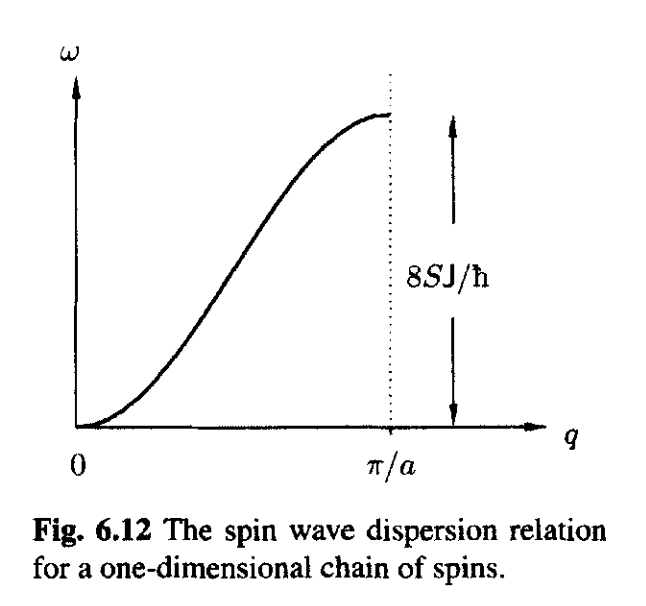
\includegraphics[height=6cm]{micm-6.12.png}
            \end{subfigure}
            \hfill
            \caption{Magnon dispersion plot from <<Magnetism in condensed matter>>.}
            \label{fig:micm-6.12}
        \end{figure}
    \end{quote}
    For the cubic system eq.~\ref{eq:micm-6.20} will look like:
    \begin{equation}
        \hbar\omega = 12JS(1 - \dfrac{1}{3}(\cos(q_xa) + \cos(q_ya) + \cos(q_za)))
    \end{equation}
    If it is to be rewritten with the notation of this paper it will look like ($n = 6$)
    \begin{equation}
        \hbar\omega = 2nJS(1 - \dfrac{1}{3}(\cos(k_xl) + \cos(k_yl) + \cos(k_zl)))
    \end{equation}

\subsection{<<Magnetisation oscillations and waves>>\cite{gurevich1996magnetization}}
    The derivation of magnon dispersion for the ferromagnet is discussed in the section~$7.4$~<<Elements of microscopic spin-wave theory>>.

    The definition of the Hamiltonian is provided on page~$205$ in equations~\eqref{eq:moaw-7.82}~and~\eqref{eq:moaw-7.82}

    \begin{quote}
        \begin{equation}
            \hatH = \gamma\hbar\sum_{f}\hat{S}_f^z - \sum_f\sum_{f^{\prime} \ne f} I_{ff^{\prime}}\mathbf{S}_f\mathbf{S}_{f^{\prime}} \label{eq:moaw-7.82} \tag{7.82}
        \end{equation}
        where $\mathbf{S}_f\mathbf{S}_{f^{\prime}} = \hat{S}_f^x\hat{S}_{f^{\prime}}^x + \hat{S}_f^y\hat{S}_{f^{\prime}}^y + \hat{S}_f^z\hat{S}_{f^{\prime}}^z$.
    \end{quote}
    The double counting is present in this Hamiltonian, thus, it is the same definition as in eq.~\eqref{eq:hh-main} of this paper with the following notation change:
    \begin{equation}
        \begin{matrix}
            f \rightarrow i, & 
            f^{\prime} \ne f \rightarrow j, & 
            I_{ff^{\prime}} \rightarrow J, & 
            \mathbf{S}_f \rightarrow \mathbf{S}_i, &
            \mathbf{S}_{f^{\prime}} \rightarrow \mathbf{S}_j
        \end{matrix}
    \end{equation}

    The dispersion law is provided in equation~\eqref{eq:moaw-7.99} on page~$209$
    \begin{quote}
        where $r_g = r_f - r_{f^{\prime}}$, $I_g \equiv I_{ff^{\prime}}$, and the last sum is over all lattice points except one, the initial. 
        The Hamiltonian ($7.98$) has the desired form of ($7.84$), and
        \begin{equation}
            \varepsilon_k(k) = \gamma\hbar H + 2S \sum_g [1 - exp(\iu \mathbf{k}\mathbf{r}_g)]I_g. \label{eq:moaw-7.99} \tag{7.99}
        \end{equation}
    \end{quote}

    For the cubic ferromagnet the textbook provides the figure~7.13 (Fig.~\ref{fig:moaw-7.13})
    \begin{quote}
        \begin{figure}[H]
            \centering
            \begin{subfigure}[b]{0.49\textwidth}
                \centering
                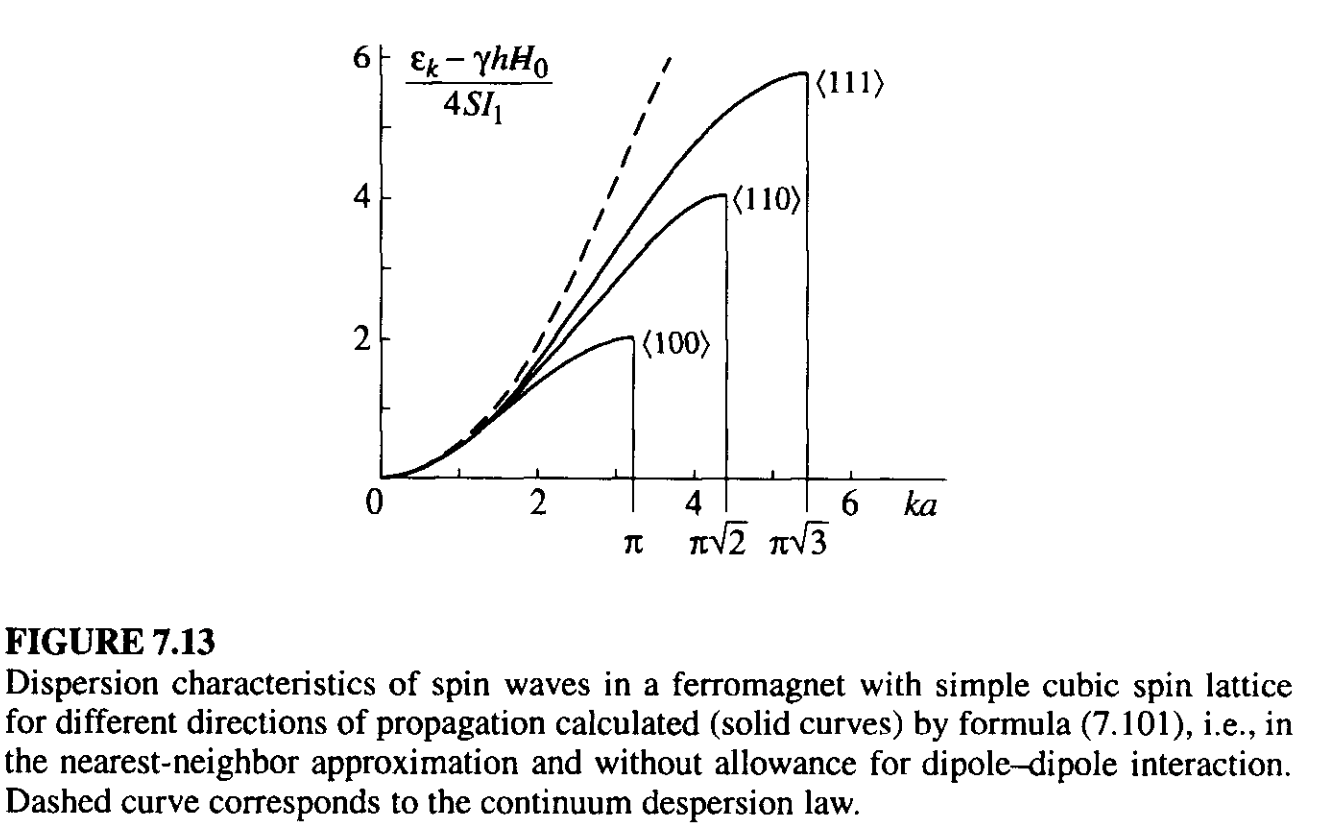
\includegraphics[height=6cm]{moaw-7.13.png}
                \caption{Original plot}
                \label{fig:moaw-7.13-original}
            \end{subfigure}
            \hfill
            \begin{subfigure}[b]{0.49\textwidth}
                \centering
                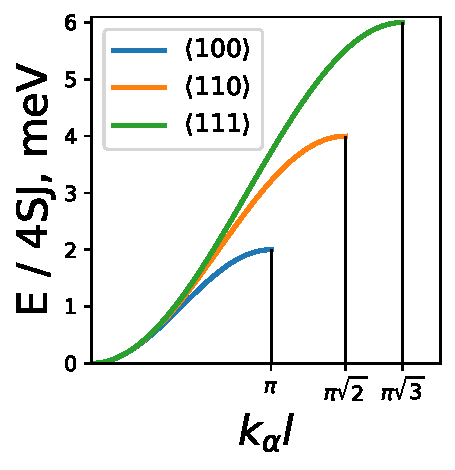
\includegraphics[height=6cm]{custom-moaw.pdf}
                \caption{Same plot with use of eq.~\eqref{eq:main-dispersion}}
                \label{fig:moaw-7.13-custom}
            \end{subfigure}
            \hfill
            \caption{Magnon dispersion plot from <<Magnetisation oscillations and waves>>.}
            \label{fig:moaw-7.13}
        \end{figure}
    \end{quote}
    In this picture curve~$\langle 100\rangle$ (from $0$ to $\pi$) corresponds to the path $\Gamma$-Y, 
    curve~$\langle 110\rangle$ (from $0$ to $\pi\sqrt{2}$) to the path $\Gamma$-M and
    curve~$\langle 111\rangle$ (from $0$ to $\pi\sqrt{3}$) to the path $\Gamma$-R 
    in the Fig.~\ref{fig:main-dispersion}. In Fig.~\ref{fig:moaw-7.13-custom} the same graph is plotted by using the equation for magnon dispersion from this paper.

    The dispersion law from eq.~\ref{eq:moaw-7.99} for the cubic system will be
    \begin{equation}
        \hbar\omega(\mathbf{k}) = 2SIn\left(1 - \dfrac{1}{3}\left(\cos(k_xr_x) + \cos(k_yr_y) + \cos(k_zr_z)\right)\right)
    \end{equation}
    where $g$ varies from $1$ to $6$ $r_g \in [r_x, -r_x, r_y, -r_y, r_z, -r_z]$ and $I_g = I$ for each $g$. 

    In the notation of this paper the dispersion law becomes ($n = 6$)
    \begin{equation}
        \hbar\omega(\mathbf{k}) = 2SJn\left(1 - \dfrac{1}{3}\left(\cos(k_xl) + \cos(k_yl) + \cos(k_zl)\right)\right)
    \end{equation}

\subsection{<<The Oxford Solid State Basics>>\cite{simon2013oxford}}
    The derivation of magnon dispersion for the ferromagnet is discussed in the exercise~$20.3$ for the Chapter~$20$~<<Spontaneous Magnetic Order: Ferro-, Antiferro-, and Ferri-Magnetism>>.

    The definition of the Hamiltonian is provided on page~$229$ in equations~\eqref{eq:ossb-20.6}~and~\eqref{eq:ossb-20.2}

    \begin{quote}
        Consider the Heisenberg Hamiltonian
        \begin{equation}
            \hatH = -\dfrac{1}{2}\sum_{\langle i,j \rangle} J \mathbf{S}_i \cdot \mathbf{S}_j + \sum_i g\mu_B \mathbf{B} \cdot \mathbf{S}_i \label{eq:ossb-20.6} \tag{20.6}
        \end{equation}
        and  for this exercise set $\mathbf{B} = 0$.
    \end{quote}

    For the first time Heisenberg Hamiltonian is defined on pages~$225-226$ in equation~\eqref{eq:ossb-20.2}
    \begin{quote}
        Note that we have included a factor of $1/2$ out front to avoid overcounting, since the sum actually counts both $J_{ij}$ and $J_{ji}$ (which are equal to each other).

        $\langle ... \rangle$

        One can use brackets $\langle i,j\rangle$ to indicate that $i$ and $j$ are neighbors:
        \begin{equation}
            \hatH = -\dfrac{1}{2}\sum_{\langle i,j \rangle} J_{ij} \mathbf{S}_i \cdot \mathbf{S}_j
        \end{equation}
        In a uniform system where each spin is coupled to its neighbors with the same strength, we can drop the indices from $J_{i,j}$ (since they all have the same value) and obtain the so-called \textit{Heisenberg Hamiltonian}
        \begin{equation}
            \hatH = -\dfrac{1}{2}\sum_{\langle i,j \rangle} J \mathbf{S}_i \cdot \mathbf{S}_j \label{eq:ossb-20.2} \tag{20.2}
        \end{equation}
        and  for this exercise set $\mathbf{B} = 0$.
    \end{quote}

    The double counting is present in this Hamiltonian, thus, it is the same definition as in eq.~\eqref{eq:hh-main} of this paper 
    with the additional factor of $1/2$, thus if we assume that definition of <<The Oxford Solid State Basics>> and this paper give the same Hamiltonian one have to 
    introduce the following substitution of exchange parameter in order to move to the definition of this paper:
    \begin{equation}
        J \rightarrow 2J \label{eq:ossb-sub}
    \end{equation}

    The dispersion law for the cubic system is provided  on page~$230$
    \begin{quote}
        $\triangleright$ Show that the dispersion curve for <<spin-waves>> of a ferromagnet is given by $\hbar\omega = \vert F(\mathbf{k})\vert$  where
        \begin{equation}
            F(\mathbf{k}) = g\mu_b\vert B \vert + JS\left(6 - 2\left(\cos(k_xa) + \cos(k_ya) + \cos(k_za)\right)\right)
        \end{equation}
        where we assume a cubic lattice
    \end{quote}

    In the notation of this paper (with the substitution~\eqref{eq:ossb-sub}) the dispersion law becomes ($n = 6$)
    \begin{equation}
        \hbar\omega(\mathbf{k}) = 2JSn\left(1 - \dfrac{1}{3}\left(\cos(k_xl) + \cos(k_yl) + \cos(k_zl)\right)\right)
    \end{equation}
\subsection{<<Magnetism and magnetic materials>>\cite{coey2010magnetism}}
    The derivation of magnon dispersion for the ferromagnet is discussed in the section~$5.4.1$~<<Spin waves>>.

    The definition of the Hamiltonian is provided on page~$137$ in equation~\eqref{eq:mamm-5.24}

    \begin{quote}
        When there is a lattice, the Hamiltonian$^1$ is generalized to a sum over all pairs of atoms on lattice sites $i, j$:
        \begin{equation}
            \hatH = -2\sum_{i > j} J_{ij} \mathbf{S}_i \cdot \mathbf{S}_j \label{eq:mamm-5.24} \tag{5.24}
        \end{equation}
    \end{quote}

    In this definition there is no double counting ($i > j$), but there is a factor of $2$ present, thus exchange constant of the Hamiltonian~\eqref{eq:mamm-5.24} are the same as in~\eqref{eq:hh-main}
    and final results for magnon dispersion are directly comparable.

    The dispersion law for the cubic system is provided  on page~$163$
    \begin{quote}
        The generalization to a three-dimensional cubic lattice with nearest-neighbour interactions is
        \begin{equation}
            \hbar \omega_q = 2JS\left[Z - \sum_{\delta}\cos\mathbf{q\cdot\delta}\right],
        \end{equation}
        where the sum is over the $Z$ vectors $\mathbf{\delta}$ connecting the central atom to its nearest neighbours.
    \end{quote}
    In case of the cubic system there is $6$ nearest-neighbours with the vectors 
    \begin{equation}
        \begin{matrix}
            (l, 0, 0),& (0, l, 0),& (0, 0, l),\\
            (-l, 0, 0),& (0, -l, 0),& (0, 0, -l),\\
        \end{matrix}
    \end{equation}
    And the dispersion law becomes:
    \begin{equation}
        \hbar \omega_q = 2JSZ\left(1 - \dfrac{1}{3}\left(\cos(q_xl) + \cos(q_yl) + \cos(q_zl)\right)\right),
    \end{equation}
    which is the same as~\eqref{eq:main-dispersion}.

\subsection{<<Rare earth magnetism>>\cite{jensen1991rare}}
    The derivation of magnon dispersion for the ferromagnet is discussed in the chapter~$5$~<<Spin waves in the ferromagnetic heavy rare earths>>.

    The definition of the Hamiltonian is provided on page~$186$ in equation~\eqref{eq:rem-5.2.1}

    \begin{quote}
        \begin{equation}
            \hatH = \sum_i\left[\sum_{l = 2,4,6}B^0_lQ_l^0(\mathbf{J}_i) + B^6_6Q_6^6(\mathbf{J}_i) - g\mu_B \mathbf{J}_i\cdot\mathbf{H}\right]
            - \dfrac{1}{2} \sum_{i\ne j} \mathcal{J}(ij)\mathbf{J} _i\cdot\mathbf{J}_j\label{eq:rem-5.2.1} \tag{5.2.1}
        \end{equation}
    \end{quote}
    
    In the equation~\eqref{eq:rem-5.2.1} crystal field and magnetic field are considered in the first sum, while the second term represents Heisenberg Hamiltonian.
    There is a double counting in the sum, thus, it is the same definition as in eq.~\eqref{eq:hh-main} of this paper 
    with the additional factor of $1/2$, therefore if we assume that definition of <<Rare earth magnetism>> and this paper give the same Hamiltonian one have to 
    introduce the following substitution of exchange parameter in order to move to the definition of this paper:
    \begin{equation}
        \mathcal{J} \rightarrow 2J \label{eq:rem-sub}
    \end{equation}

    The spin-wave spectra is defined on the page~$190$ in the equation~\eqref{eq:rem-5.2.22}
    \begin{quote}
        The energy parameters are
        \begin{equation}
            \begin{matrix}
                U_1 = \dfrac{1}{2}\sum_{\mathbf{q}}(E_{\mathbf{q}} - A_{\mathbf{q}}); & E_{\mathbf{q}} = \sqrt{A_{\mathbf{q}}^2 - B^2}.
            \end{matrix}
            \label{eq:rem-5.2.22} \tag{5.2.22}
        \end{equation}
    \end{quote}
    where $A_{\mathbf{q}}$, $A$ and $B$ are defined in the equations~\eqref{eq:rem-5.2.18} and~\eqref{eq:rem-5.2.15}
    \begin{quote}
        \begin{equation}
            \begin{matrix}
                A = \dfrac{1}{J}\left\{3B^0_2J^{(2)} - 21B^6_6J^{(6)}\cos6\phi + g\mu_BJH\cos(\phi - \phi_H)\right\}\\
                B = \dfrac{1}{J}\left\{3B^0_2J^{(2)} + 15B^6_6J^{(6)}\cos6\phi\right\}.
            \end{matrix}
            \label{eq:rem-5.2.15} \tag{5.2.15}
        \end{equation}

        $\langle ... \rangle$

        
        \begin{equation}
            A_{\mathbf{q}} = A + J\left\{\mathcal{J}(\mathbf{0}) - \mathcal{J}(\mathbf{q})\right\}
            \label{eq:rem-5.2.18} \tag{5.2.18}
        \end{equation}
    \end{quote}
    $A = 0$ and $B = 0$ if there is no magnetic field nor anisotropic effects are considered. In the case of this paper $L = 0$, thus $J = S$ and the equation for the dispersion law is
    \begin{equation}
        E_{\mathbf{q}} = S\mathcal{J}(\mathbf{0}) - \mathcal{J}(\mathbf{q})
    \end{equation}

    $\mathcal{J}(\mathbf{q})$ is defined in the equation~\eqref{eq:rem-5.1.1a}
    \begin{quote}
        \begin{equation}
            \begin{matrix}
                \mathcal{J}_{ss\prime}(\mathbf{q}) = \sum_{j \in s^{\prime} - subl.} \mathcal{J}(ij)e^{-\iu\mathbf{q}\cdot(\mathbf{R}_i - \mathbf{R}_j)}; & i \in s-sublattice,
            \end{matrix}  
            \label{eq:rem-5.1.1a} \tag{5.1.1a}
        \end{equation}
    \end{quote}
    And for the cubic lattice it becomes:
    \begin{equation}
        \mathcal{J}(\mathbf{q}) = J \left(e^{-\iu k_xl} + e^{\iu k_xl} + e^{-\iu k_yl} + e^{\iu k_yl} + e^{-\iu k_zl} + e^{\iu k_zl}\right) = 2J \left(\cos(k_xl) + \cos(k_yl) + \cos(k_zl)\right)
    \end{equation}
    And the dispersion law becomes:
    \begin{equation}
        E_{\mathbf{q}} = S(6J - 2J \left(\cos(k_xl) + \cos(k_yl) + \cos(k_zl)\right))
    \end{equation}
    In the notation of this paper after the substitution~\eqref{eq:rem-sub} formula for the dispersion law is ($n = 6$)
    \begin{equation}
        E_{\mathbf{q}} = Sn2J(1 - \dfrac{1}{3} \left(\cos(k_xl) + \cos(k_yl) + \cos(k_zl)\right))
    \end{equation}

     





    \bibliographystyle{plain} 
    \bibliography{refs.bib} 



    % \section*{References}
    % \printbibliography[title = {\vspace{-2em}}]



\end{document}
